\subsection{距離センサーを使ってみよう}
距離センサーをHSPで使ってみましょう。距離センサー(番号は書いてありません。\ref{distance}ページを参考にしてください)をA0につなげましょう。HSPスクリプトエディタで、/home/pi/ome/05/kyori.hspを開いて実行してください。
\begin{figure}[H]
  \begin{minipage}[t]{0.3\columnwidth}
    \centering
 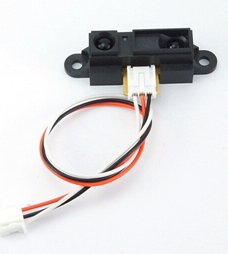
\includegraphics[width=\linewidth]{images/chap05/text05-img031.png}
    \caption{距離センサー}
  \end{minipage}
  %\hspace{0.01\columnwidth} % ここで隙間作成
  \begin{minipage}[t]{0.5\columnwidth}
    \centering
    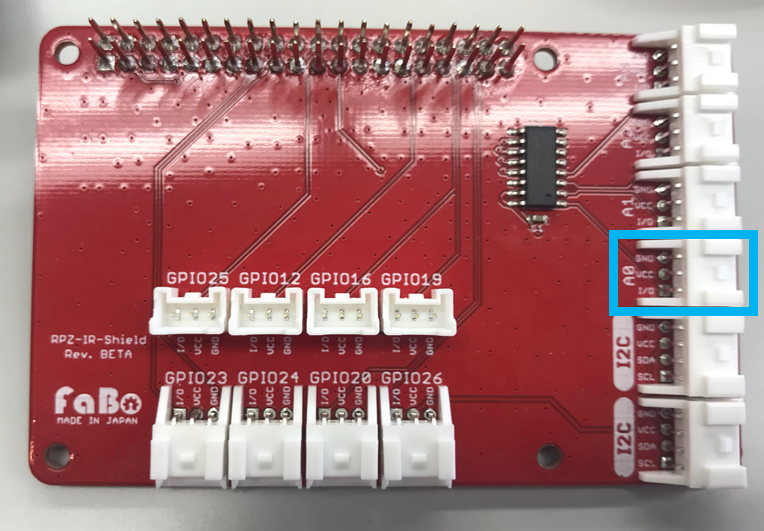
\includegraphics[width=\linewidth]{images/chap05/text05-img030.png}
    \caption{A0}
  \end{minipage}
\end{figure}

\begin{lstlisting}[caption=kyori.hsp,label=kyori.hsp]
#include "hsp3dish.as"
#include "rpz-gpio.as"

spiopen 0	<#blue#;SPIチャンネルを開く#>

*main

	data = spiget(0,0)	<#blue#;SPIを使ってデータを受け取る#>
	kyori = -1*(data*5000/1023)/36+845/9	<#blue#;dataを距離に変換する#>
	res = "距離 : "+kyori
	
	redraw 0
	font "",20
	pos 30,30
	mes res
	redraw 1

	wait 10
	goto *main

spiclose 0	<#blue#;SPIチャンネルを閉じる#>
\end{lstlisting}

データは\code{spiget}を使って受け取ることができます。値は0~1023になります。これでは距離がわからないので、受け取った値を距離に変換する必要があります。変換するための式は\ref{distance}ページに書いてあります。今回は入力は\code{data}という変数にしているので、式のxをdataにします。\code{kyori = -1*(data*5000/1023)/36+845/9}で入力を距離に変換し、\code{kyori}変数に代入しています。単位はcmです。\\

\begin{tcolorbox}[title=\useOmetoi]
\begin{enumerate}
\item 距離センサーをA0につなげてkyori.hspを実行してみましょう。距離はだいたい10~80cmです。
\end{enumerate}
\end{tcolorbox}